\documentclass[12pt,a4paper]{article}
\usepackage{amsmath}
\usepackage{amsfonts}
\usepackage{amssymb}
\usepackage{polski}
\usepackage{indentfirst}
\usepackage{graphicx}
\usepackage{natbib}
\usepackage{verbatim}
\usepackage{commath}
\usepackage{url}
\usepackage{hyperref}
\usepackage[margin=1in]{geometry}

\begin{document}

\title{Analiza i Przetwarzanie Dźwięku - Sprawozdanie z projektu 1.}
\author{Szymon Tomulewicz}
\date{6 IV 2020}
\maketitle
\tableofcontents
\newpage

\section{Wprowadzenie\label{sec:wprowadzenie}}
Celem projektu było stworzenie aplikacji okienkowej, umożliwiającej wczytywanie plików wav,
a następnie analizowanie ich pod kątem wybranych parametrów i wartości.

\subsection{Aplikacja\label{sec:aplikacja}}
Aplikacja została wykonana w języku C\#, przy użyciu biblioteki NAudio do przetwarzania i analizy plików dźwiękowych, oraz biblioteki WinForms do stworzenia interfejsu oraz wyświetlania parametrów. Wybrałem NAudio ze względu na popularność tej biblioteki, ilość dokumentacji oraz integrację z biblioteką WinForms.

Aplikacja składa się z jednego widoku (Rys. \ref{fig:app_preview}), na którym po załadowaniu pliku dzwiękowego rysują się wykresy parametrów opisanych w dalszej części sprawozdania.

\begin{figure}[h!]
\centering
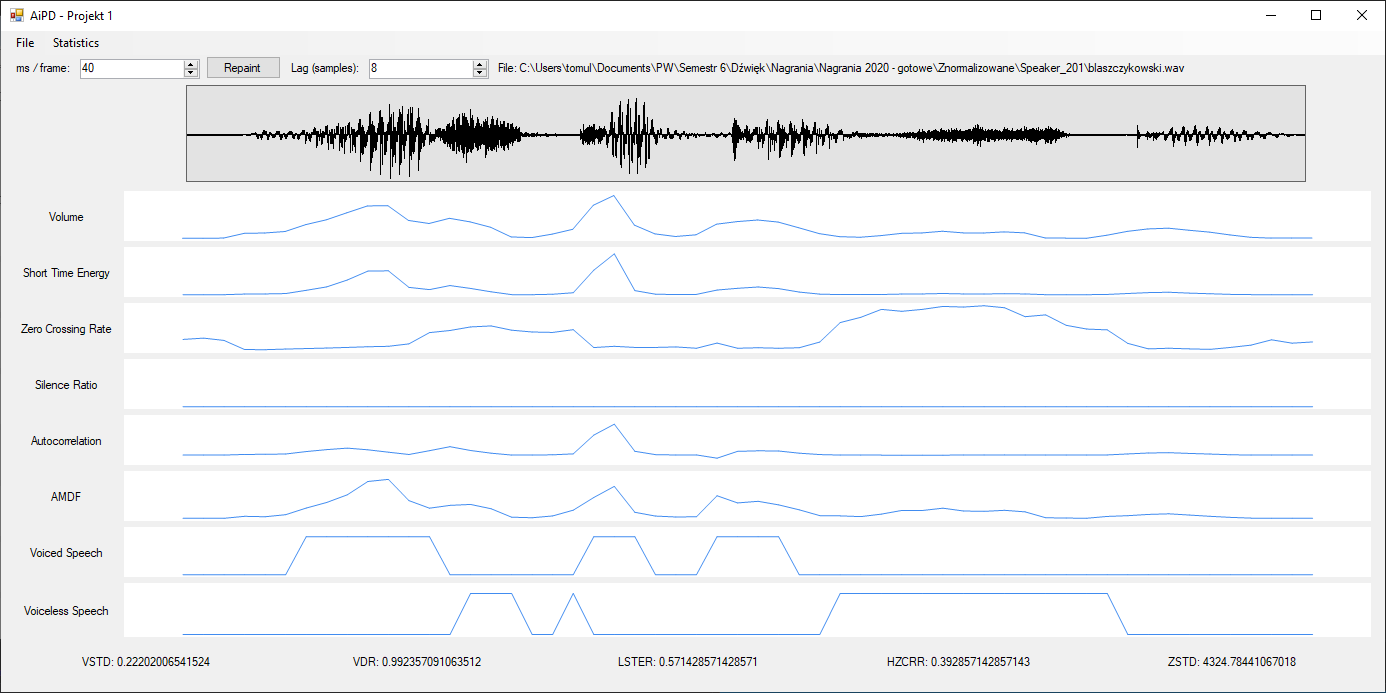
\includegraphics[width=1.0\textwidth]{figures/app_preview}
\caption{Przykładowy stan aplikacji}
\label{fig:app_preview}
\end{figure}

Użytkownik może podać w interfejsie dwie wartości: długość ramki w milisekundach oraz parametr (tzw. \emph{lag}) używany w funkcji autokorelacji oraz AMDF (Average Magnitude Difference Function). Jako jednostkę parametru \emph{lag} aplikacja przyjmuje liczbę próbek.

\section{Obliczane parametry\label{sec:parametry}}
Wszyskie obliczenia w aplikacji, które są wykonywane na próbkach, używają typów zmiennoprzecinkowych.
NAudio umożliwia to przy użyciu metody \verb|ToSampleProvider|:

\begin{verbatim}
    using (WaveFileReader reader = new WaveFileReader(filePath))
    {
        // Convert to 32-bit floating point samples:
        ISampleProvider sampleProvider = reader.ToSampleProvider();
        ...
        float[] buffer = new float[frameSizeFloats];
        ...
        sampleProvider.Read(buffer, 0, frameSizeFloats);
        ...
    }
\end{verbatim}

\subsection{Parametry w dziedzinie czasu na poziomie ramki (Frame-level)\label{sec:framelevel}}
Parametry opisane w kolejnych sekcjach są obliczane, a następnie zapisywane i wyświetlane w formie wykresów (Rys. \ref{fig:app_preview}). $N$ występujace we wzorach oznacza zwykle długość ramki w próbkach.

\subsubsection{STE - Short Time Energy\label{sec:ste}}
Dla n-tej ramki, $STE$ wynosi:
\begin{equation}
    STE(n)=\frac{1}{N}\sum_{i=0}^{N-1}s_n^2(i)
\end{equation}
Gdzie $s_n(i)$ to amplituda i-tej próbki w n-tej ramce.

\subsubsection{Volume - głośność\label{sec:volume}}
Dla n-tej ramki, głośność wynosi:
\begin{equation}
    v(n)=\sqrt{STE(n)}
\end{equation}

\subsubsection{ZCR - Zero Crossing Rate\label{sec:zcr}}
Dla n-tej ramki, $ZCR$ wynosi
\begin{equation}
    Z(n)=\frac{1}{2}\bigg(
        \sum_{i=1}^{N-1} \abs{sign(s_n(i))-sign(s_n(i-1))}
    \bigg)\frac{f_s}{N}
\end{equation}
Gdzie $sign$ to funkcja signum, a $f_s$ to częstotliwość próbkowania sygnału.

\subsubsection{Częstotliwość tonu podstawowego\label{sec:f0}}
W nadziei na możliwość obliczenia tonu podstawowego zaimplementowałem obliczanie następujących funkcji:
\begin{itemize}
\item
    Funkcji autokorelacji:
    \begin{equation}
        R_n(l)=\sum_{i=0}^{N-l-1}s_n(i)s_n(i+l)
    \end{equation}
\item
    Funkcji AMDF (Average Magnitude Difference Function):
    \begin{equation}
        A_n(l)=\sum_{i=0}^{N-l-1}\abs{s_n(i+l)-s_n(i)}
    \end{equation}
\end{itemize}
Gdzie $s_n(i)$ oznacza amplitudę i-tej próbki w n-tej ramce, a $l$ - parametr $lag$ podany przez uzytkownika.

Niestety dla tych parametrów, operacja obliczania (a właściwie przybliżania) częstotliwości tonu podstawowego okazała się zbyt kosztowna (Zob. \cite{leszczyna}) na potrzeby tego projektu.

\subsection{Cechy sygnału audio na poziomie klipu (Clip-level)\label{sec:cliplevel}}
Parametry opisane w kolejnych sekcjach są obliczane, a następnie zapisywane i wyświetlane na dole widoku (Rys. \ref{fig:app_preview}).

\subsubsection{VSTD\label{sec:vstd}}
Odchylenie standardowe znormalizowane przez maksymalną wartość głośności w całym klipie.
\begin{equation}
    VSTD=\frac{1}{max(v)}\sqrt{
        \sum_{n=0}^{F}\big(
            v(s_n) - avg(v)
        \big)^2
    }
\end{equation}
Gdzie $F$ jest liczbą ramek, na które został podzielony klip, $v(s_n)$ - głośnością w n-tej ramce, $max(v)$ - maksymalną wartością głośności w całym klipie, a $avg(v)$ - średnią głośnością w całym klipie.

\subsubsection{ZSTD\label{sec:zstd}}
Analogicznie liczone jest odchylenie standardowe $ZCR$. W tym wypadku jednak aplikacja nie normalizuje otrzymanej wartości.
\begin{equation}
    ZSTD=\sqrt{
        \sum_{n=0}^{F}\big(
            z(s_n) - avg(z)
        \big)^2
    }
\end{equation}
Gdzie $z(s_n)$ jest wartością $ZCR$ w n-tej ramce, a $avg(z)$ - średnią wartością $ZCR$ w całym klipie.

\subsubsection{VDR - Volume dynamic range\label{sec:vdr}}
\begin{equation}
VDR=\frac{max(v)-min(v)}{max(v)}
\end{equation}
Gdzie $max(v)$ to maksymalna głośność w klipie, a $min(v)$ - minimalna.

\subsubsection{LSTER - Low Short Time Energy Ratio\label{sec:lster}}
\begin{equation}
    LSTER=\frac{1}{2N}\sum_{n=0}^{N-1}[
        sgn(0.5*avg(STE)-STE(n)+1
    ]
\end{equation}
Gdzie $N$ to całkowita liczba ramek, $avg(STE)$ - średnia wartość $STE$ w jednosekundowym oknie, a $STE(n)$ - wartość $STE$ w n-tej ramce.

\subsubsection{HZCRR - High Zero Crossing Rate Ratio\label{sec:hzcrr}}
\begin{equation}
    HZCRR=\frac{1}{2N}\sum_{n=0}^{N-1}[
        sgn(ZCR(n)-1.5*avg(ZCR))+1
    ]
\end{equation}
Gdzie $N$ to całkowita liczba ramek, $avg(ZCR)$ - średnia wartość ZCR w jednosekundowym oknie, a $ZCR(n)$ - wartość $ZCR$ w n-tej ramce.

\section{Wykrywanie ciszy\label{sec:silent}}
Aplikacja wykrywa ciszę w klipie audio przy pomocy wcześniej obliczonych wartości ZCR oraz głośności. Dla każdej ramki, sprawdzane są poziomy tych wartości. Jeśli $v(n) < 0.02$ oraz $Z(n) < 50$, sygnał w danej ramce uznawany jest za ciszę.
\begin{verbatim}
    // Dla każdej ramki
    for (int n = 0; n < frameCount; n++)
    {
        // 1.0 -> cisza
        double value =
            (volumeData[n] < 0.02 && zcrData[n] < 50.0) ? 1.0 : 0.0;
        // Dodaj do wykresu
        dt.Rows.Add(n, value);
    }
\end{verbatim}
Metoda ta nie jest doskonała, co zostanie pokazane w sekcji \ref{sec:prezentacja}.

\section{Wykrywanie mowy dźwięcznej i bezdźwięcznej\label{sec:mowa}}
Określanie mowy dźwięcznej i bezdźwięcznej jest możliwe z dość dużym przybliżeniem przy użyciu $STE$ oraz $ZCR$ (\citep{bachu08}). Jako materiał pomocny w przybliżaniu progów użyłem znormalizowanych nagrań z poprzednich lat. Finalnie warunki jakie muszą być spełnione żeby dany sygnał audio w ramce został zakwalifikowany jako
\begin{itemize}
    \item Mowa bezdźwięczna: $STE(n)<0.03 \land z(n) \ge 6000$
    \item Mowa dźwięczna: $STE(n)\ge0.03 \land z(n) < 6000$
\end{itemize}
Dokładność tej metody zostanie pokazana w sekcji \ref{sec:prezentacja}.

\section{Prezentacja wyników działania\label{sec:prezentacja}}
Może dla kilku różnych parametrów, na różnych sygnałach żeby można było porównać

%- w sprawozdaniu porównać dla róźnych nagrań i opisać
%  - różnego typu nagrania (najlepiej np. audycje radiowe, też nagrania naszych głosów)
%  - Porównanie wyników dla różnych nagrań: radio (mowa + muzyka), mowa (głos męski, żeński), muzyka
%  - Określenie fragmentów muzyka / mowa
%  - wgrać np fragment audycji radiowej spróbować określić gdzie jest muzyka gdzie mowa (nie proste przy tych parametrach pewnie przybliżone)

\section{Wnioski\label{sec:wnioski}}
Na podstawie wyników (i implementacji) można napisać wnioski. Np.:

\subsection{Napotkane problemy\label{sec:problemy}}
Domyślne wykresy, jakie oferuje biblioteka WinForms okazały się dalekie od oczekiwań jakie możnaby mieć w projekcie takim jak ten. Nie udało mi się niestety dostosować ich na tyle, aby czytelne były zarówno wykresy, jak i wartości je opisujące. W kolejnych projektach planuję wypróbować inne biblioteki do rysowania wykresów.

Kolejną trudnością, jaką napotkałem i której nie udało mi się rozwiązać, było wczytywanie plików mp3. Brak płynności w nomenklaturze związanej zarówno z NAudio, jak i formatami plików audio okazał się dość dużą barierą.

\subsection{Czy metoda zawsze działa dobrze? Dla wszystkich przypadków?\label{sec:}}
Czy metoda zawsze działa dobrze? Dla wszystkich przypadków?

\subsection{Czy parametry można zmieniać dowolnie? Może są poprawne tylko w jakimś zakresie.\label{sec:}}
Czy parametry można zmieniać dowolnie? Może są poprawne tylko w jakimś zakresie.

\subsection{Dlaczego są różne wersje? Czy któraś jest lepsza?\label{sec:}}
Dlaczego są różne wersje? Czy któraś jest lepsza?

\section{Zakończenie\label{sec:zakonczenie}}
Zakończenie.

\bibliographystyle{plain}
\bibliography{references}
\end{document}
